\documentclass{grattan}


% Comments are deployed by the % sign; everything after % is ignored by the compiler.
% Please do not put comments before \documentclass as these are reserved for TeX directives.
% add_to_dictionary: SSBs i ii iii CESE AYP RCTs frontline pay-offs ATAR judgments


\addbibresource{bib/GonskiSub.bib}

%Note from CC: All refs should go in GonskiSub.bib for now. 

\author{Julie Sonnemann and Peter Goss}
\title{The Commonwealth’s role in improving schools}

\GrattanReportNumber{2018-02}

\ReportOrWorkingPaper{Report}

\acknowledgements{%
This Report was written by Julie Sonnemann and Peter Goss.

We would like to thank the members of Grattan Institute's School Education Program Reference Group for their helpful comments, as well as numerous government and industry participants and officials for their input.

The opinions in this report are those of the authors and do not necessarily represent the views of Grattan Institute's founding members, affiliates, individual board members reference group members or reviewers.
Any remaining errors or omissions are the responsibility of the authors.

Grattan Institute is an independent think-tank focused on Australian public policy.
Our work is independent, practical and rigorous.
We aim to improve policy outcomes by engaging with both decision-makers and the community.

For further information on the Institute's programs, or to join our mailing list, please go to: \textcolor{blue}{\url{http://www.grattan.edu.au/}}.

{\footnotesize
This report may be cited as: 
Sonnemann, J. and Goss, P\@. (2018). \emph{\mytitle}. Grattan Institute.

ISBN: 978-0-6482307-2-4

All material published or otherwise created by Grattan Institute is licensed under a Creative Commons Attribution-NonCommercial-ShareAlike 3.0 Unported License\par
}
}


\begin{document}

\begin{overview}
Australia needs a new national conversation on school education. We should seize the opportunity provided by the Commonwealth's Review to Achieve Educational Excellence in Australian Schools (known as the `Gonski 2.0 Review'). 

The Turnbull Government commissioned the Gonski 2.0 Review in an effort to ensure the extra Commonwealth money going into schools over the next decade is spent wisely by the states and territories. But this report warns against over-reach: too much Commonwealth intervention into school education could be counterproductive and costly.

Under the Gonski 2.0 funding deal struck last year, schools will get an extra \$23 billion in Commonwealth funds over the next ten years. 
But the Commonwealth's need for reassurance about how the money is spent must be kept in perspective: the extra federal funding is only 3 per cent of all government spending on schools over the period. 

Much more important is that all government money for school education is spent effectively, regardless of where it comes from. This report first identifies the big system reforms needed to improve students outcomes. Most of these reforms are the responsibilities of state and territory governments. Then the report considers what few things the Commonwealth should do to help. 

The biggest advances will be made only if Australia adopts a more `adaptive' school education system. Neither a top-down nor a bottom-up model of governance is desirable. Instead, schools need more support to ensure teachers know what works in the classroom, and how they can adapt their teaching methods to better meet the needs of their students. This requires a much greater focus on student progress, and on how teachers use data to evaluate and target their teaching. Teachers need more opportunities to develop and get feedback from their colleagues, along with more guidance on tried and tested classroom materials to reduce `reinvention of the wheel'.

Driving any of these big reforms from Canberra would be difficult. Imposing prescriptive funding conditions on states and territories can destroy policy coherence and simply increase red tape. The Commonwealth has few ways to independently verify if change is actually happening in the classroom, and adding an extra layer of government policies that chop and change only disrupts schools and teachers. The Turnbull Government's 2016 Quality Schools Quality Outcomes policy -- which includes a long list of over 15 potential new national requirements -- is a big step in the wrong direction. 

Instead we recommend the Commonwealth focus strategically on a few national reforms. Given the difficulties in Commonwealth-state relations, it is far better to focus on a few actions with a high chance of success and strong buy-in from state governments. The Commonwealth should abandon any policy `reform' that does not meet all three criteria: evidence shows it is a good idea; government can make it happen; and Commonwealth intervention will help. 

We nominate four areas likely to succeed as national reforms: invest in measuring new, 21st century skills; develop betters ways to measure student progress; invest in high-quality digital assessment tools for teachers; and create a new national research organisation to share what works best.

The extra Commonwealth money for schools under Gonski 2.0 is welcome. But for Australian students to get the most benefit, the Commonwealth must resist the temptation to over-reach by intervening heavily in school education policy.

\end{overview}

\contentspage
\listoffigures

\begin{recommendations}


%\chapter{Policy recommendations}\label{chap:Policy-recommendations}

In pursuit of national reform in school education, the Commonwealth Government should:

\begin{itemize}
    \item \textbf{First, deliver fully on existing Commonwealth responsibilities before embarking on new national initiatives.} The federal government's role in initial teacher education, delivering a rigorous national curriculum, improving national assessments, and embedding the professional standards all require constant attention, and some require urgent reform. 
    
    \item \textbf{Recognise that many of the big reforms are the responsibility of the system managers; that is, the state and territory governments.} The Commonwealth must collaborate with the states and territories on any new national efforts; state and territory `buy-in' is essential.
    
    \item \textbf{Select a small number of national reforms (only) and do them well.} Given the difficulties in driving improvement from Canberra, avoid spreading efforts too thinly. 
    
     \item \textbf{Prioritise the reforms most likely to succeed as national reforms.} We suggest three key criteria:
     
     
    (i) Is it a good idea?
    
    (ii) Can government make it happen?
    
    (iii) Will Commonwealth intervention help?
    
    \end{itemize}
   
\newpage
 
Specifically, the Commonwealth Government should consider the following four reforms that meet the above criteria:
    
    \begin{enumerate}
   
    \item \textbf{Invest nationally to improve how we measure non-cognitive and critical thinking skills.} There is a big need for research in this area, and it should be done in collaboration with states and territories.
    
    \item \textbf{Develop new national measures of learning progress} for diagnostic use in the classroom, and for national bench-marking in collaboration with state and territory curriculum and assessment authorities.
    
    \item \textbf{Invest in high-quality digital tools to help teachers regularly assess classroom learning} alongside a new `star rating' system to help schools when searching for the most appropriate assessment tools.
    
    \item \textbf{Establish a new national independent evidence body} to help identify national priorities, set rigorous standards of evidence, fund high-quality research (especially randomised controlled trials) and disseminate and promote findings. This body could link-up various strands of research on education for people from birth through to age 18.
    
   \end{enumerate}
   

\end{recommendations}


    
   







\chapter{The context: new national school reforms are likely in 2018}\label{chap:National-reform-context}

The Gonski 2.0 Review comes at a critical time. Australia’s educational performance is declining internationally, we face new challenges in preparing students for future work, and equity gaps are too wide. 

The time is ripe for a discussion on the Commonwealth Government’s role as it negotiates a new agreement on school funding with the states and territories later this year. 

This report argues that the Commonwealth should not have a much bigger role in schooling than it does today. Federal Government over-reach could do considerable damage. 

\section{The Gonski 2.0 Review will help inform the Commonwealth's next steps}\label{sec:Commonwealth-next-steps}

The Turnbull Government wants to ensure that its promised extra \$23 billion of schools funding is spent wisely. The extra federal money was announced in 2017 as part of new funding arrangements (known as `Gonski 2.0') that seek to better align funding to student need. The Commonwealth and state and territory governments are currently negotiating the terms of the new funding agreement that spans over ten years from 2018-2027.

The Gonski 2.0 Review has been commissioned in this context. The review team has been asked to examine the evidence on what works in schools and school systems, as well institutional, governance, transparency and accountability measures required to ensure what works is implemented. The review team has received numerous public submissions.\footnote{All submissions, including Grattan Institute's, are due to be made public once the Gonski 2.0 Review team has delivered its final report.}

\section{New federal conditions on funding could be on the table}\label{sec:Commonwealth-influence}

Under constitutional arrangements, state and territory governments are responsible for ensuring the delivery and regulation of schooling.

However the federal government can exert greater control over schooling policy through Section~96 of the Constitution which allows for conditions on Commonwealth funding to state and territory governments. 

The current federal government has sent some signals that it could seek to use the Gonski 2.0 Review findings to impose new conditions and increase its influence over school education policy.

The federal Department of Education and Training has stated that the Review will `\textit{make sure that reform actions are based on a solid understanding of what works}' and that `\textit{implementation of reforms will be a condition of funding for states}'.\footcite{DETQualitySchoolsFrequentlyAskedQuestions}

And the Commonwealth’s 2016 strategic document Quality Schools, Quality Outcomes includes about 15 new input and output reforms that state and territory governments could be required to implement.\footcite{2016AustralianGovernmentQualitySchoolsQualityOutcomes} 
For example, it suggests focusing on reforms `requiring teachers to use explicit literacy and numeracy instruction in schools' (the list of reforms is included in \Chapref{chap:New_initiatives_quality_schools}).\footnote{The status of these reforms is still unclear, because the Education Council typically needs to agree for them to have standing.}

\section{New requirements are not desirable}\label{sec:Commonwealth-actions-can-have-unintended-consequences}

If the Commonwealth does choose to impose new input and output conditions, this would be a significant departure from recent approaches to Commonwealth-state relations and would run counter to the learnings from the 2014 White Paper series on federal reform.\footnote{The White Paper process documented learnings from past Commonwealth-state reform efforts and explored ways to improve federal financial relations in Australia.} 

Schools and states should be held accountable for students' educational progress and ensuring that money is spent wisely.\footnote{This refers not only to government education departments but also Catholic and independent schools.}
But the Commonwealth should tread warily when seeking to increase accountability to themselves rather than the public. If federal policy makers pull the wrong levers, the consequences can be very damaging. 

The Commonwealth should keep its desire to expand control in check. The promised extra Commonwealth funds are only 3 per cent of all government spending on schools from 2018 to 2027. It is important to ensure that \textit{all} government money invested in schools is well spent – and most of that money is provided by state and territory governments.

The overall reform agenda, for which states and territories are primarily responsible, should focus on the changes that will really shift the dial, rather than the sub-set of issues that the Commonwealth can achieve.

\section{The structure of this report}\label{sec:The-big-national-conversation}

The next two chapters explain the big reforms in school education in Australia, many of which are within state and territory responsibilities. \Chapref{chap:Design_an_adaptive_system_of_continuous_improvement} describes the adaptive system design settings needed to achieve continuous improvement in schools, and highlights the need for more systemic support to help frontline professionals embed evidence in daily practice. \Chapref{chap:Specific-reforms} identifies specific system reforms that could make a big difference, drawing on previous Grattan Institute work. 

The remaining chapters discuss what role the Commonwealth should play in this broader reform agenda. \Chapref{chap:Commonwealth-conditions} argues the Commonwealth should refrain from prescriptive new conditions. \Chapref{chap:few-reforms} explains how the Commonwealth should prioritise only a small number of national reforms, in close collaboration with states and territories. \Chapref{chap:what_com_should_do} recommends four specific national reforms the Commonwealth should collaborate on to benefit students across the nation.

Lastly, Early childhood education is outside of the scope of the Gonski 2.0 review and not discussed in this report, but should be a high priority for national reform given its big impact on student outcomes, especially for disadvantaged children. Many children are behind or at risk when they start school, and many never catch-up. 



\chapter{The big reform agenda: creating an adaptive education system design}\label{chap:Design_an_adaptive_system_of_continuous_improvement}

This chapter discusses how to achieve a system of continuous school improvement, and the broader system settings needed to help teachers to know what works best for their students and how they can translate this into daily classroom practice. 

A top-down model is not sufficient for sustained improvement. But neither is a bottom-up system, with 10,000 schools doing their own thing. 

A strong evidence base on `what works' is just the beginning: many other factors also need to be in place for teachers to embed evidence in their classroom practice. A more `adaptive' system design is needed, with stronger feedback loops for more systematic learning.

\section{Create a more adaptive education system}\label{sec:Create-a-more-adaptive-education-system}

School education in Australia faces three big challenges: 

\begin{itemize}
    \item First, we must improve the teaching of core foundational skills, where the challenge is largely about how to spread what works best. 
    \item Second, we need to better prepare young people in `new' capabilities in critical thinking and non-cognitive capabilities, where we know little about what works best.
    \item Third, we must address the large gaps between advantaged and disadvantaged groups.
\end{itemize}

The system must be designed to cater to each of these very different challenges. It needs to encourage teachers to embed clear, existing evidence where it exists (for example on core foundational skills), and at the same time enable disciplined innovation where the evidence is weak (for example in critical thinking and non-cognitive skills). An adaptive education system gives adequate direction to teachers, but also ensures they are equipped to make sound judgments where there is ambiguity.%
\footnote{For further discussion see the Grattan Institute report, Towards an adaptive education system in Australia (\textcite{Goss2017TowardsAnAdaptiveSystem}).}

Adaptive improvement is best thought of as an iterative, deliberate way to learn by doing, using a feedback loop with an explicit focus on inputs and outcomes as well as the learning processes along the way. Adaptive reform uses data to link what is done (inputs) to what is learnt (outcomes) and systematically improve the learning process over time. An adaptive system ensures that all parts of the system promote learning.


\begin{figure}
\caption{The Grattan Institute model shows how to use feedback loops to improve education outcomes\label{fig:Grattan-Institute-Model}}
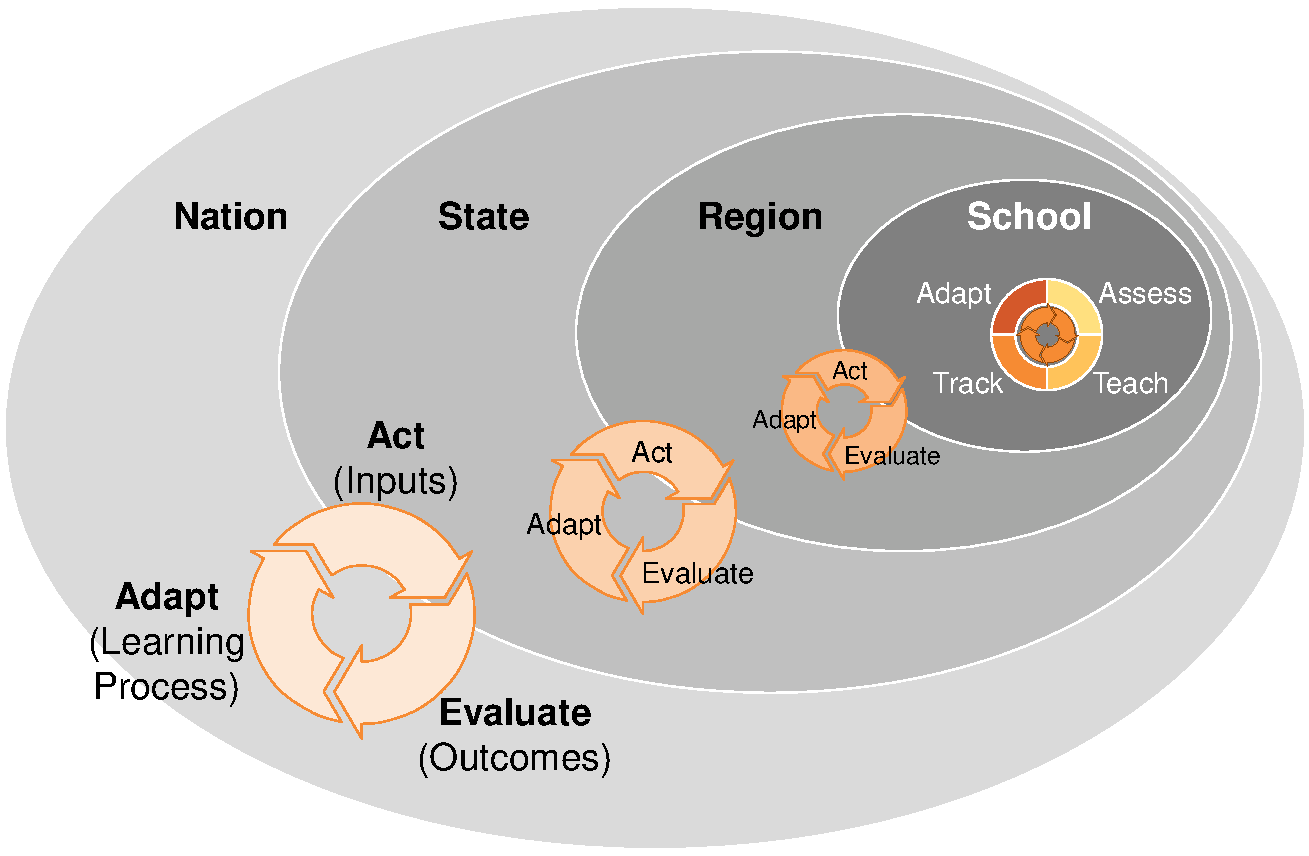
\includegraphics[page=1]{charts/GonskiReportCharts.pdf}
\source{\textcite{Goss2017TowardsAnAdaptiveSystem}
Note the school level feedback loop of `assess, teach, track and adapt' embeds the idea of targeted teaching which is at the heart of adaptive improvement.}
\end{figure}



\section{Strengthen feedback loops at multiple levels}\label{sec:Strengthen-feedback-loops-at-multiple-levels}

School education has been much slower than other professions such as medicine and engineering to produce scientific evidence and incorporate it into practice. Even where the evidence is clear, it is not necessarily taken up. This is not only an issue in schools, but also in government policy making.  

An adaptive education system has strong evaluative structures and feedback loops to help embed evidence in practice. \Vref{fig:Grattan-Institute-Model} depicts such a system, with feedback loops at four levels: school, region, state, and nation. 

At a minimum there are three steps in any feedback loop: (i) `Act' by deliberately selecting inputs or programs to meet needs; (ii) `Evaluate' by tracking and measuring the outcomes; and (iii) `Adapt' by using learnings on what worked best to inform actions next time around.

Feedback mechanisms can encourage a more evaluative way of working, but a range of other barriers to using evidence need to be overcome too. The next sections discuss some of those barriers.




\begin{figure}
\caption{There are many possible reasons people do not use evidence in practice\label{fig:There-are-many-possible-reasons-people-do-not-use-evidence-in-practice}}
\includegraphics[page=2]{charts/GonskiReportCharts.pdf}
\source{Adapted from \textcite{ProductivityCommission2016NationalEvidenceBase}}
\end{figure}


\section{Better understand why people use evidence (or don’t)}\label{sec:Better-understand-why-people}

%ERROR
There are many possible reasons schools and policy makers do not use evidence in daily decisions, as shown in \Vref{fig:There-are-many-possible-reasons-people-do-not-use-evidence-in-practice}.
%
Research findings need to be readily accessible, timely, relevant and trustworthy. The organisational culture must support risk-taking. Individuals must possess the skills to translate and implement the evidence. Interaction between researchers and public servants can be beneficial, including at the departmental level.



\subsection{System-level policies can increase the uptake of evidence}\label{subsec:System-level-policies-can-increase-the-uptake-of-evidence}

Government policies can increase the use of evidence in daily decisions, but there is little high-quality research on exactly what system policies and programs are most effective. 

Studying high-performing education systems can shed some light on the types of policies likely to help in spreading evidence. Some OECD research points to a mix of policies for system-wide improvement and behaviour change in schools, including both vertical and horizontal accountability, as well as capacity building initiatives.%
\footcite{BurnsKoster2016GoverningEducation}

School education literature includes some research on the conditions that facilitate `adult learning' and improvement, but more is needed.\footnote{For a summary of the research on how adults `learn' professionally, see \textcite{Jensen2016PDTeacherProfessional}.}
One common theme is that collaboration and professional learning communities can play a big role in shifting attitudes (when done well), because it encourages deep conversations among practitioners that can challenge existing beliefs over time. Other qualitative literature suggests school improvement is not so much about changing mindsets as changing behaviours.\footcite{Macklin2017DrivingSchoolImprovement}
It suggests routines can be a powerful tool to get teachers to change behaviour. They first experience the benefits for student learning, which then influences a shift in mindset later on. The Productivity Commission has identified this as an issue for further research in Australia.\footcite{ProductivityCommission2016NationalEvidenceBase}

`Improvement' science can help shed light on what school settings are needed to translate evidence into practice. It involves researchers working directly with educators to adapt evidence to local needs and solve specific problems of practice. This collaborative structure can help persuade sceptical educators that scientific research is relevant to their specific context.

But improvement science is not a system-wide solution; large-scale improvement will only come with better-designed experiments that also incorporate steps on how to actually implement the practice under investigation, including the guidance or system supports needed.%
  \footcite{Dynarski2015UsingresearchtoimproveeducationundertheEveryStudentSucceedsAct}
This is the focus of the growing field of implementation science research.%
  \footnote{Implementation science is slightly different to improvement science; it studies the methods and approaches to help update and integrate research findings into routine practice.}

The Gonski 2.0 Review team should synthesise the existing research on how best to implement what works. It should explore research in:

\begin{itemize}
    \item Literature from school education, psychology, public policy, management, organisational change, improvement science and implementation science. 
    \item System design in high-performing school education systems, including the system-level policies and programs for spreading evidence-based practice.\footcite{Jensen2012CatchingUpLearning}
    \item Other professional sectors, including nursing, medicine, engineering and aviation.
\end{itemize}

Such research will be useful for schools, but also for policy makers in designing the system-level policies and structures most likely to improve classroom teaching. 

The next chapter identifies more specific system-level reforms that can help build a more adaptive education system. 



\chapter{Big reforms will deliver real improvements}\label{chap:Specific-reforms}

This chapter outlines a number of big reforms at the system level that will help embed the use of evidence in schools. They include focusing more on student progress (growth) rather than achievement at a point in time, and improving teaching effectiveness and school leadership. Policy makers also need to gather better data on what is actually happening inside schools.

Critically, most of the big reforms are in areas of state and territory government responsibilities. This is not surprising given they are the system managers of schools.

\section{Focus more on student progress (growth)}\label{sec:Focus-more-on-student-progress-growth}

School education policy should explicitly aim to improve the progress (growth) of all students, not just their achievement at a point in time. This requires:

\begin{itemize}
    \item Putting more `small data' on student progress in the hands of teachers so they can improve teaching in the classroom; and
    \item Putting better `big data' on student progress in the hands of policy makers so they can monitor the system more effectively.
    
\end{itemize}

Small data should be the first priority, because this is known to have one of the biggest impacts on the effectiveness of teaching. Teachers should better use classroom data to track the progress of each of their students, and adapt their teaching to suit what each student is ready to learn next. 

Unfortunately, this is not the norm in Australian schools, as we discussed in our 2015 report, Targeted Teaching.\footcite{Goss2015TargetedTeachingHow}
Student achievement varies by up to seven years in a typical Year 9 classroom in Australia.\footcite{Goss2016Wideninggapswhat}
To better use data in practice, teachers need more tools, training, trust, time and team work (as discussed in \Vref{subsec:strengthen_the_use_assessment}).

Australia must improve how it measures student progress both on core academic skills and `new' capabilities such as critical thinking and non-cognitive skills (the latter issue is discussed in \Chapref{chap:what_com_should_do}). 

\section{Improve teaching effectiveness}\label{sec:Improve-teaching-effectiveness}

Effective teaching has the largest impact on student learning outside of the home environment.\footnote{Discussed in \textcite{Jensen2010Investinginourteachers}.} But too often we talk about teacher quality as though the individual teacher is the point at issue. No teacher is an island; teachers need more support from the system. Six specific proposals are suggested in the following sections, drawing on past Grattan reports. 

\subsection{Prioritise teacher time and standardise some elements of practice}\label{subsec:prioritise} 

Teacher time is an expensive and precious resource. But simply giving teachers more time will not necessarily lead to better teaching and learning. Teacher time must be redirected from low-impact to high-impact activities. This means relieving teachers of administrative activities. But it also means more standardisation of daily teaching practices.\footnote{The first issue is discussed in \textcite{Jensen2012Makingtimeforgreatteaching} and the second issue in \textcite{Goss2015TargetedTeachingHow}.} 

In particular, more use of high-quality, tried and tested support materials can enhance student learning and reduce `reinvention of the wheel'. Standardisation could include more common lesson plans and formative assessments, more guidance on which textbooks to use and how to use them, and careful use of educational technology. 

Policy makers and school leaders must lift their game: they make many of the critical decisions on teachers' use of time.  

\subsection{Strengthen the use of assessment data}\label{subsec:strengthen_the_use_assessment}
Three changes should be made to help teachers use data more effectively to improve their teaching.\footnote{Discussed in \textcite{Goss2015TargetedTeachingHow}.}

First, teachers should get better guidance on how to interpret data on student progress and then adapt their teaching. This is not just about more `data managers' in schools, but more specialised pedagogical guidance to help translate the data into instructional steps. It’s the dialogue that matters, not the data.

Second, teachers should get more and better classroom assessment tools and resources. Such tools should be aligned to the curriculum, easy to use, and provide guidance on how to use data to adjust teaching. Australia needs better tools to measure foundational skills in all subject domains (not just literacy and numeracy) as well as `new' capabilities in critical thinking and non-cognitive outcomes.

Third, government should help teachers to evaluate the tools available, for example by introducing a `star rating' system. Too often, schools and teachers choose their tools based on trial and error, anecdote or a Google search.

\subsection{Make collaborative learning more productive}\label{subsec:collaborative-learning}

Collective teacher efficacy has one of the largest effects on student learning.\footcite{Hattie2015Whatworksbestineducation}
But simply working in a group is not enough, as seen in the US where there have been huge investments with little returns.\footcite{TNTP2015TheMirage}
Australia needs much better ways for teachers to collaborate, moving beyond the simple exchanging of lesson plans to deeper discussions on instruction, interpreting data, and integrating evidence into new ways of working. High-performing education systems such as Shanghai, Singapore and Hong Kong show the way, with their focus on `professional learning communities', including valuable input from expert teachers who guide group discussions.\footnote{Discussed in \textcite{Jensen2012CatchingUpLearning}.}   

\subsection{Improve feedback and appraisal}\label{subsec:feedback}

Feedback is one of the most powerful ways to improve teaching practice.\footnote{Discussed in \textcite{Jensen2011BetterTeacherAppraisal}.}   And it doesn't cost much. Teachers need feedback about their strengths and weaknesses if they are to improve their teaching. But many in Australia don’t get that information during professional learning, appraisal, or their performance management.

\subsection{Strengthen student engagement}\label{subsec:engagement}

As many as 40 per cent of students in Australia are unproductive in a given year, and these students learn less over time.\footnote{Discussed in \textcite{Gossetal2017Engagingstudents}.}
Teachers find this very stressful and are calling out for more support. We must provide better initial training and in-school support in managing classes, as well as better research on the root causes of the problem.
\subsection{Redesign the workforce so that top teachers spread best practice}\label{subsec:specialist-teachers}

Our best teachers can help lift the effectiveness of the whole workforce. Yet they often remain isolated, with heavy teaching loads in their own classrooms.\footnote{Discussed in \textcite{Pete-2016-theOz-School-funding-circuit-breaker-with-appeal-to-all}.}
In high-performing systems, such as Shanghai and Singapore, an elite cohort of specialist teachers sets the direction for effective practice and spreads the message via cross-school networks.\footnote{Discussed in \textcite{Jensen2012CatchingUpLearning}.}  

Australia’s top teachers have some of these functions on paper, but they rarely get to enact them in their schools, or across schools.\footnote{Some Australian states have more stringent policies on how senior teachers are used in schools; for example, Queensland's new `master teachers' are expected to develop teachers across schools.} While the Australian Professional Standards for Teachers have been an important step in introducing the roles of Highly Accomplished and Lead Teachers (HALT) who develop other teachers in schools, these roles are not the norm in most schools today.

State and territories should introduce new `master teacher' and `expert teacher' roles for teachers who are specialists in their subject areas to address this issue. Such positions would not only build workforce capacity but elevate the importance of subject-specific teaching expertise.\footnote{These positions have two important differences to the roles of Highly Accomplished and Lead Teachers (HALT) in the Australian professional standards: 1) they are both subject-specific, and 2) the master teacher role works across schools. Ideally these features should be embedded in the HALT role descriptions in the national standards.}

\section{Revamp school leadership pathways}\label{sec:revamp-leadership}

School leaders are critical to school improvement, yet Australia doesn't select or properly train people well for these roles. School principal shortages will become much worse unless the career path is made clearer and more attractive. Singapore is a shining example: it identifies outstanding leaders early,  provides them with intensive training (a six-month, full-time program), and follows up with strong peer-network support.\footnote{Discussed in \textcite{Jensen2012CatchingUpLearning}.}

\section{Strengthen the evidence base and data flows}\label{sec:evidence-base}

Australia needs to improve how it produces and disseminates evidence on what works in classrooms.\footnote{Discussed in \textcite{Goss2016SubmissiontotheProductivityCommissionInquiryintotheNationalEducationEvidenceBase}.}
In particular, we need to:
\begin{itemize}
    \item Lift the standards for scientific evidence, and produce more randomised controlled trials and quasi-experimental studies. Major government policies should be better evaluated, and more funding provided for longitudinal studies to identify trends over time. Establishing nationally agreed scientific evidence standards would be a good first step. 
    \item Conduct better research on the conditions that encourage teachers to use the evidence on what works.
    \item Better synthesise, translate and share research findings so they are readily accessible to educators and policy makers across the country.
    \item Build the research capacity of schools and policy makers through specialised training and support
    
\end{itemize}

In addition, the network of state-based education research institutions should be strengthened. Research could be shared more widely across states, along with better national coordination of major research efforts to avoid duplication and gaps. 

The analytic capabilities of state based research bodies could also be improved. For example the NSW Centre for Education Statistics and Evaluation (CESE) was established in 2012 to improve the effectiveness, efficiency and accountability of education in NSW\@. Its work informs education funding in NSW, by determining what works and where investment will have the most impact. 

\subsection{Better understand what is happening in schools}\label{subsec:practices}

Education policy makers cannot ensure money is spent well if they do not know what is actually happening in schools. In Australia, too little is known about which pedagogical methods are being used, or the nature of collaboration in schools. As a consequence it is difficult to identify problems, formulate solutions and evaluate results.\footnote{The Victorian Auditor-General has raised this issue, see \textcite{2010Auditor-General}.}   

\section{Emerging reforms to explore}\label{sec:emerging}

The following reforms could hold promise and should be explored further:

\begin{itemize}
    \item Redesigning Initial Teacher Education, so fewer people are trained more intensively (as done in Singapore).\footnote{Discussed in \textcite{Jensen2012CatchingUpLearning}.} This could produce better outcomes for no extra cost. 
    \item Increasing the use of high-quality textbooks and programs of curriculum content, so individual teachers do not have to `reinvent the wheel'.\footcite{Koedel2017Bigbangforjustafewbucks} 
    \item Expanding the use of student feedback, which has been shown to be a reliable indicator of teaching quality.\footcite{MET2012AskingStudentsAboutTeaching}
    \item Training teachers in how to use technology to enhance their teaching, especially in subjects such as maths where there could be large benefits.
    \item Tackling teacher shortages in maths, science and IT, through salary increases and by training existing teachers to give them specialist capabilities.\footcite{ProductivityCommission2017Shiftingthedial}
    \item Boosting incentives to attract high-performing teachers to disadvantaged schools.\footnote{Discussed in \textcite{Riceetal2017Howtogetqualityteachersindisadvantagedschools}.}
    
\end{itemize}


\section{What governments should not do}\label{sec:governments-not-do}

We recommend against an even greater focus on targets, or teaching standards and regulations. 
Targets are useful in agreeing on priorities, but can divert resources from important but less visible activities. Similarly, teaching standards and regulations help to guarantee minimum quality but are unlikely to significantly enhance workforce development.

It is also dangerous to rely too much on school autonomy, transparency, accountability and choice as key levers for improvement.\footnote{Discussed in \textcite{Jensen2013Themythsofmarkets}.}
In particular, the evidence shows that increasing school autonomy will not get the desired results in the absence of the right system support for schools.\footcite{Suggett2015SchoolautonomyNecessarybutnotsufficient}


\chapter{New Commonwealth conditions are not the way to go}\label{chap:Commonwealth-conditions}

This chapter argues that the Commonwealth should have only a modest role in the big reform agenda to improve school education. It should refrain from expanding its control over school spending. Prescriptive Commonwealth funding conditions have been tried before for little benefit. They can create confusion and tend to result in tick-a-box responses. 

\section{We must learn from history}\label{sec:learn-from-history}

The 2008 Council of Australian Governments (COAG) reform agenda was an attempt to leave behind the old bureaucratic processes. It produced the National Education Agreement, which introduced national performance benchmarking, professional teaching and leadership standards, and a national curriculum. A number of these initiatives were successful, and many were rigorously evaluated, adding to the knowledge base on what works. But there were many costs related to input and output control elements that outweighed the benefits.\footnote{The COAG reform agenda was a shift to outcomes-based federal conditions, however as the reform agenda rolled out there was more of a focus on inputs and processes than intended.}

The 2014 Federation White Paper process documented some of these failings.%
\footcite{2014AustralianGovernmentReformoftheFederationWhitePaper}
It called for a better allocation of roles and responsibilities to make it easier for governments to identify what the problems are in education and who is responsible for fixing them -- and for the public to identify who is accountable.\footcite{2014AustralianGovernmentReformoftheFederationWhitePaper}
It said confusion about accountability can arise where state and territory governments focus on reporting to the Commonwealth rather than to their constituents.

The White Paper series pointed to increased red tape and wasteful duplication of effort.\footcite{2014AustralianGovernmentReformoftheFederationWhitePaper} Onerous reporting also increases the regulatory burden, an issue for both federal and state governments that can outweigh any benefits gained. 

When states are not on board, they tend to give `tick-a-box' responses, going through the motions of complying without actually enforcing real change. An international review highlighted that the lack of state government buy-in to Australia's COAG reform processes was a significant barrier to making the collaborative effort work.\footcite{HowesEngele2013WhytheCOAGReformAgendaHasFloundered, HowesEngele2013FederalReformStrategies}

A key lesson is that policy coherence can be compromised where policy levers are dispersed between Commonwealth and state governments. The involvement of an additional tier of government can create confusion for teachers, schools and systems, especially if policies and funding arrangements chop and change.

\section{Alternative forms of Commonwealth control do not have clear benefits}\label{sec:other-approaches}

Tying federal government funding to national outcomes-based indicators, with punishment for states that fail to meet targets, can also have damaging consequences. For example, the US `No Child Left Behind' policies led to some perverse outcomes for few gains (see \Vref{box:US-approaches-to-federal-accountability}).

Nor should the federal government establish new `quality assurance frameworks', given the fraught status of Commonwealth-state relations. The US federal government has adopted a quality assurance approach under The Every Student Succeeds Act (ESSA) (2015), demanding states show the extent to which their policies and programs are evidence-based. It is too early to assess its success (see \Vref{box:US-approaches-to-federal-accountability}). But in Australia, such an approach would increase red tape, and the states and territories would be likely to regard it as a threat to their turf.

\begin{bigbox}{US approaches to federal accountability}{box:US-approaches-to-federal-accountability}

\textbf{No Child Left Behind, 2001 onwards}

The No Child Left Behind (NCLB) policy was introduced with bi-partisan support in 2001, but had such calamitous consequences that there was also bipartisan support for its abolition in 2014.

Under NCLB, the federal government demanded that all states each year test 95 per cent of their students between years 3 and 8 in reading and maths. Schools were punished if they were judged not to have met their (state set) targets on `Adequate Yearly Progress' (AYP). Punitive actions included restructuring of the school, or allowing and encouraging parents to send their children to other schools.

This top-down, high-stakes testing approach created perverse incentives.\footnote{Discussed in \textcite[][39]{Goss2015TargetedTeachingHow}.}
For example, state governments began lowering their standards when setting their AYP targets. Teachers began narrowing the curriculum to prepare their students for the tests in reading and maths.\footcite{Jacob2010TheImpactofNoChildLeftBehind}
Some schools discouraged students from participating in the tests. Some schools and teachers resorted to desperate measures to alter test records.
By the end, there was unanimous support for reinventing federal policies and abandoning high-stakes testing.

\textbf{The Every Student Succeeds Act (ESSA) (2015)}

ESSA reduces federal control by moving away from demanding high-stakes accountability to demanding states show that their policies and programs are evidence-based.

Under ESSA, all states are still required to monitor and test 95 per cent of their students, but the federal government now allows states to develop their own system of accountability for underperforming schools.

States must show that they have evidence-based plans and interventions to address underperformance. There is an agreed national framework for what constitutes `evidence'.

ESSA reduces the punitive consequences for schools not making adequate progress, and will avoid most of the perverse incentives created under NCLB\@. But it is too early to say whether these policy changes will result in improved education outcomes in the US\@. 

\end{bigbox}


\chapter{The Commonwealth should prioritise a small number of national reforms}\label{chap:few-reforms}

\Chapref{chap:Commonwealth-conditions} highlighted the dangers of using new federal funding conditions to drive education reform. This chapter argues that the Commonwealth should pursue a small number of reforms (at most) that have a high chance of success. It outlines criteria that should be used to assess potential Commonwealth reforms.

\section{Screen reforms through a prioritisation process}\label{sec:screen-reforms}

Developing an integrated approach for even one major reform effort is hard work. Trying to implement a long list of reforms means efforts are likely to be too thinly spread to improve practice in the classroom -- the ultimate goal.

\begin{figure}
\caption{The Commonwealth should intervene only if a reform proposal meets these three criteria}\label{fig:criteria-to-determine-if-proposed-reforms}
\includegraphics[page=3]{charts/GonskiReportCharts.pdf}
\end{figure}

We propose a prioritisation framework with three criteria for identifying a small number of reforms with a high chance of success (see \Vref{fig:criteria-to-determine-if-proposed-reforms}). The three criteria are: 

\begin{itemize}
    \item Is it a good idea? There should be strong evidence that the core concept of the proposal will have a big and positive impact on student outcomes, and can address a big problem in the Australian system in reasonable time and at reasonable cost. 
    \item Can government make it happen? There should be expert consensus that government intervention can make a difference, with the right system settings, policies and/or programs to help bring the idea into practice.
    \item Will Commonwealth intervention help? The idea must be amenable to Commonwealth oversight and monitoring. Benefits such as national scale, filling a gap, and policy consistency, should be weighed against costs such as duplication, displacement of state priorities, policy incoherence, and red tape. State `buy-in' to the problem and solution is critical for the collaborative effort to work.   

\end{itemize}



\section{Conditions are often costly and hard to impose}\label{sec:conditions-fall-down}

Many proposed Commonwealth controls may look like a good idea in theory; that is, they may meet the conditions set out in criterion 1 (Is it a good idea?). But most tend to fall down on criterion 2 (Can government make it happen?) and criterion 3 (Will Commonwealth intervention help?). In particular, it is difficult for the Commonwealth\space government to adequately monitor the controls from Canberra, and there are confusion and costs from an extra layer of government involvement. 

Commonwealth requirements that simply mandate a specific `evidence-based practice' are unlikely to lead to much practical change. State and territory governments can rarely just flick a switch to implement a Commonwealth directive.

The Commonwealth may not know that elements in the delivery chain might be missing at the state level. Simply requiring one new initiative is unlikely to deliver change if other state-level policies are not aligned to support it.

\subsection{The `requiring explicit teaching in schools' example}\label{subsec:explicit-teaching}

In its Quality Outcomes Quality Schools 2016 strategy, the Commonwealth Government said it intended to require \textit{``explicit teaching in schools''}.\footcite{2016AustralianGovernmentQualitySchoolsQualityOutcomes} While `explicit teaching' is strongly backed by evidence (although not as an exclusive strategy), it would be a poor policy choice for the Commonwealth.

First, there is not yet any common understanding of what `explicit teaching' would involve, or exactly how different it would be from current practice.

Second, state governments are unlikely to have the right mix of policies and programs to help teachers switch to `explicit teaching'. States do not have a good track record in scaling evidence-based practice. For example, the right professional learning, school structures, accountability processes, and incentives all need to be in place.

Third, it is not clear that the Commonwealth is best-placed to lead this change. It would be difficult, for example, for the Commonwealth to independently monitor and verify changes in teaching practice, given little data is collected on teaching practices in schools.

Finally, there would be costs arising from the confusion in adding a federal policy at odds with state policies. A federal requirement mandating a certain practice would be inconsistent with the policy approach of most states, which is to devolve decisions on pedagogy to schools.

Regardless of whether mandating `explicit teaching' is a good policy, enforcing it from the Commonwealth level would create policy incoherence and could create confusion in regions and schools. 


\chapter{What the Commonwealth should do next}\label{chap:what_com_should_do}

This chapter details what the federal government should do in collaborative national efforts to ensure that education money is spent well. The Commonwealth’s biggest focus should be on delivering effectively in areas within its existing remit. Beyond that, the Commonwealth should do four specific things that would fill genuine gaps in Australia’s school education system. 

The proposed new national reforms should only be pursued if the states `buy in' and there is sustained Commonwealth-state collaboration in design and delivery.

\section{Deliver on existing federal responsibilities first}\label{sec:deliver-responsibilities}
The Commonwealth\space government can make significant contributions to school education through its existing areas of responsibility. It plays a large role in training teachers. The national curriculum, national student testing, high-quality data collection, and implementing professional standards in schools are all critical to the functioning of schools. All require constant attention, and some require urgent reform.

For example, the Commonwealth has much to do in improving initial teacher education, in line with recommendations of a major review in 2013.\footcite{2015AustralianGovernmentActionNowClassroomReadyTeachersReport}
A 2014 departmental review of the Australian Curriculum and Reporting Authority (ACARA) called for major changes to the National Report on Schooling.\footcite{2014AustralianGovernmentReviewoftheAustralianCurriculum}
And a 2016 Productivity Commission report on the National Evidence Base highlighted the important role the federal government plays in high-quality national data collection.\footcite{ProductivityCommission2016NationalEvidenceBase}
The Commonwealth\space government should act on recommendations such as these before embarking on new interventions into school education policy.

\section{Four specific national reforms}\label{sec:four-additional}

The following four reforms meet the three criteria set out in \Chapref{chap:few-reforms}. They do not `demand' specific inputs or outputs from the states. They are areas where increased scale and coordination is likely to result in big benefits for students. 
 
\subsection{Invest in measuring `new' capabilities}\label{subsec:new-capabilities}

Agreeing on the broad educational outcomes we want is seductively easy. But measuring progress in them is not. In many cases, Australia still lacks a concrete understanding of how to even teach non-cognitive skills, such as teamwork and resilience. As a result, we focus much more on measuring narrower foundational skills of literacy and numeracy, which are only an element of what we expect from schooling.

\begin{figure}
\caption{Giving teachers more `small data' will help}\label{fig:improve-how-to-measure}
\includegraphics[page=4]{charts/GonskiReportCharts.pdf}
\end{figure}

We must invest more in how to measure broader outcomes, and especially in `small data' for teachers to use in the classroom. The potential for big improvements is illustrated in \Vref{fig:improve-how-to-measure}. 

The Commonwealth should collaborate with states and territories on a major national research effort to improve how we measure these broader 21st century skills. Developing classroom measurement tools should be the first priority.  Every state and territory faces a similar challenge in this area, so it is appropriate for the Commonwealth\space government to invest and help coordinate this project in close collaboration with states and territories.

\subsection{Develop better measures of learning progress}\label{subsec:national-measure}

Australia needs better measures of student progress for national bench-marking and for use in the classroom.

NAPLAN seeks to measure students' learning progress in core literacy and numeracy skills at the national level, but NAPLAN gain scores are not easy to interpret when comparing the progress of different student groups. The Commonwealth\space government should develop a better measure of learning progress in NAPLAN for `big data' purposes.\footnote{Discussed in \textcite{Goss2016Wideninggapswhat}.}

The Commonwealth\space government should also develop a new `small data' progress measure for teachers to use in the classroom. This could be linked to the national curriculum and create consistency on what a year of learning progress looks like (new tools in this area are discussed in the next section).%
  \footcite{Goss2016Wideninggapswhat}
A 2011 OECD review of Australian policies highlighted the need for more `small data' to enhance student assessment in the classroom.%
  \footcite{OECD2011ReviewsofEvaluationandAssessmentinEducationAustralia}

\subsection{Invest in high-quality digital assessment tools for the classroom}\label{subsec:new-digital}

A consistent measure of progress in the classroom is one thing. But the tools to assess it are another. The Commonwealth\space government should invest in high-quality digital assessment tools that measure learning progress in the classroom. Quality assessment tools help to diagnose what students know, how much progress they have made, and how teaching can be improved to better meet students' needs. Measuring impact on student learning is the key to good decisions about what to keep and stop -- the selection process at the heart of an adaptive education system (see \Chapref{chap:Design_an_adaptive_system_of_continuous_improvement}).

Such tools should examine core academic skills (including a broad range of subject areas beyond literacy and numeracy), as well as new capabilities in critical thinking and non-cognitive skills. Given the curriculum is national, it is wasteful for each state (and many schools) to develop their own classroom assessment tools.\footcite{Goss2015TargetedTeachingHow} Any national efforts to develop new tools must be in consultation and close collaboration with state curriculum and assessment authorities, who should work in partnership with ACARA.

While the Commonwealth should improve teachers' access to assessment tools, the states and territories also need to ensure teachers have the capacity to interpret and use the assessment results to adjust their teaching -- a big issue in schools. Without complementary state government effort in this area, little is likely to change in teaching practice.

The Commonwealth\space government should also develop a `star' rating system for commercial assessment tools, to help schools choose the most appropriate new tools for their needs. Assessment experts should rate new products to help reduce individual school search costs (a large hidden cost).  This function could be done by existing bodies such as Education Services Australia or ACARA with appropriate extra funding for its delivery.

\subsection{Create a new national evidence body}\label{subsec:evidence-national} 

The Commonwealth should collaborate with the states to establish a new, national, independent research body that could encourage more evidence-based decision making in school education.

This body would complement, rather than replace, the existing network of state government research bodies. The Commonwealth would collaborate with states to establish the new organisation. Its functions would include sharing research findings across the country, setting national research priorities, lifting the standards for researchers, and helping to commission more rigorous research, trials and longitudinal surveys. Australia needs more and better education research; the Commonwealth should help fund it.\footnote{Of course any nationally commissioned research would have to be agreed to by state and territory governments and go through appropriate ethics approvals.} 

The new body could link-up all research on education for people from birth through to age 18, so there is a better understanding of the continuum of key learning stages from early childhood, school education through to  vocational education.

Specifically, the new national body should:

\begin{itemize}
    \item Coordinate research priorities and plan a long-term research agenda for school education
    \item Establish national evidence standards that encourage Randomised Controlled Trials (RCTs) and quasi-experiments
    \item Oversee high-quality research, trials and longitudinal surveys on ways to improve specific practices, in collaboration with state and territories (discussed in \Chapref{chap:Design_an_adaptive_system_of_continuous_improvement})
    \item Synthesise data and research findings so they are readily accessible to schools and policy makers
    \item Promote research findings through a range of media platforms and distribution channels.
    \item Bring researchers, schools and policy makers together so they can better understand the research and how to implement its lessons. \end{itemize}

The new body could be made up of a number of specialist branches; for example, one arm could specialise in evidence production and another in promotion (as done by the US Institute of Education Sciences).

It must be independent of government, for several reasons. Foremost, an independent body would be more likely to gain the trust of the education sector and the wider community. Teachers and school leaders are tired of government policies chopping and changing. They must be confident that the work of a national evidence body will not continually change with political tides. An independent body would help minimise political interference in the research agenda.

We do not agree with the Productivity Commission that ACARA is the best fit for a national evidence body, given the potential conflict of interest with its other functions.

Of course, independence does not necessarily guarantee quality. We agree with the criteria spelled out in the 2016 Productivity Commission report for selecting the appropriate governance arm.\footcite{ProductivityCommission2016NationalEvidenceBase}  

    

    

\appendix

\chapter{Potential new initiatives in the federal Government's 2016 schools strategy}\label{chap:New_initiatives_quality_schools}

The list below is our interpretation of  potential new national requirements outlined in the federal Government's Quality Schools, Quality Outcomes strategy (2016). We understand the strategy document still requires full Education Council approval in order to be enacted so the status of some initiatives is unclear. 

Pedagogy and curriculum
\begin{itemize}
 \item Require teachers to use explicit literacy and numeracy instruction in schools
 \item Assess children in reading, phonics and numeracy during Year 1
 \item Require a minimum standard of literacy and numeracy from all students completing Year 12
 \item Require successful completion of an English or humanities subject and a maths or a science subject as a pre-requisite for students to get an ATAR
 \end{itemize}

Workforce
\begin{itemize}
 \item Mandate literacy/numeracy as a specialisation for primary teacher training
 \item Require graduate teachers to achieve registration at the Proficient level within three years of teaching
 \item Publish employment data against each level of the professional standards on My School 
 \item Set recruitment targets for STEM-qualified teachers and Indigenous teachers
 \item Find ways to improve the supply of competent language teachers
 \item Establish incentives to attract and retain experienced school leaders in disadvantaged schools
  \item Recognise high-performing teachers and reward them with increased pay
 \item Certify all new principals through a new national certification process
 \end{itemize}

Other accountability measures 
 \begin{itemize}
 \item Report annually to parents against agreed national literacy and numeracy standards
 \item Meet attendance targets, including specific targets for Indigenous students
 \item Systems that receive additional funding for disadvantage in areas such as Indigenous, low English, disability and low SES must show how the money will be used to improve outcomes 
 \item Indexation of Commonwealth funding contingent on meeting the outlined reform commitments\par
  {\footnotesize\textit{Source:}~\textcite{2016AustralianGovernmentQualitySchoolsQualityOutcomes}.\par}

\end{itemize}




\printbibliography

\end{document}







